% cd /storage/emulated/0/Documents/documents/latex/1920/Grade-10/1st/equation-and-graph-of-a-circle && pdflatex ps-equation-and-graph-of-a-circle.tex && termux-open ps-equation-and-graph-of-a-circle.pdf

% cd /storage/emulated/0/Documents/documents/latex/1920/Grade-10/1st/equation-and-graph-of-a-circle && clean-tex ps-equation-and-graph-of-a-circle-input1.tex


% cd /storage/emulated/0/Documents/documents/latex/1920/Grade-10/1st/equation-and-graph-of-a-circle && convert -density 600 ps-equation-and-graph-of-a-circle.pdf -crop 2200x1700 -quality 100 -verbose ps-equation-and-graph-of-a-circle%02d.png

%2480.5x3508 portrait 2x2 2550x3300
%3508x2480.5 landscape 2x2 3300x2550 
%1653.7x2338.7 portrait 3x3 1700x2200
%landscape 3x3 2200x1700

% cd /storage/emulated/0/Documents/documents/latex/1819/grade10/visual/4th/equation-and-graph-of-a-circle && while inotifywait -e close_write ps-equation-and-graph-of-a-circle*.tex; do touch /storage/emulated/0/Android/data/com.termux/files/launch-termux.txt && printf '1' > /storage/emulated/0/Android/data/com.termux/files/launch-termux.txt && pdflatex ps-equation-and-graph-of-a-circle.tex && termux-open ps-equation-and-graph-of-a-circle.pdf; done

% cd /host-rootfs/storage/emulated/0/Documents/documents/latex/1819/grade10/visual/4th/equation-and-graph-of-a-circle && while inotifywait -e close_write ps-equation-and-graph-of-a-circle*.tex; do pdflatex ps-equation-and-graph-of-a-circle.tex  && printf "/storage/emulated/0/Documents/documents/latex/1819/grade10/visual/4th/equation-and-graph-of-a-circle/ps-equation-and-graph-of-a-circle.pdf" > /host-rootfs/storage/emulated/0/GNURoot/home/Scripts/file-to-launch.txt; done


\documentclass[10pt]{article}
\usepackage[letterpaper, landscape, right=0.25in, left=0.25in, top=0.25in, bottom=0.25in]{geometry}
\usepackage{xcolor}
\usepackage{anyfontsize}
\usepackage{enumitem}
\usepackage{multicol}
\usepackage{amsmath}
%\usepackage{amsfonts,dsfont}% for \mathds 
\usepackage{tabularx} 
\usepackage{gensymb}
\usepackage{multirow}
\usepackage{graphicx, tipa}
\usepackage{tikz}
\usetikzlibrary{angles,quotes}
\usepackage{pgfplots} 
\usetikzlibrary{calc}
\pgfplotsset{compat=newest}
\usetikzlibrary{arrows.meta}
\usetikzlibrary{intersections}
\usetikzlibrary{decorations.pathreplacing}
\usepackage{flafter}
\usepackage{amsmath,amssymb,cancel,units}
\usepackage{microtype} % nicer output 
\usepackage{hfoldsty} % nicer output 
\usepackage{fixltx2e} 
\usepackage{mathptmx}
%\usepackage{booktabs}
\usepackage{numprint}
\usepackage[utf8]{inputenc} 
\usepackage[T1]{fontenc}
%\usepackage{siunitx} 
%\sisetup{detect-all}


\def\radA{3.6cm}

\def\radB{3.6cm}

%\def\thirdrad{8cm}

\pagenumbering{gobble}
%\linespread{0.9}
\newcommand{\vspce}{\vspace{0.75ex}}
\newcommand{\hspce}{\hspace{0.5em}}
\newcommand{\blank}{\underline{\hspace{2em}}}%{\rule{1em}{0.15ex}}
\newcommand{\arc}[1]{{% 
\setbox9=\hbox{#1}% 
\ooalign{\resizebox{\wd9}{\height}{\texttoptiebar{\phantom{A}}}\cr#1}}}

\newcolumntype{C}{ >{\centering\arraybackslash} X}




\begin{document}
\boldmath
{\fontsize{36}{40}\fontfamily{pnc}\selectfont {

\def\curdir{/storage/emulated/0/Documents/documents/latex/1920/Grade-10/3rd/equation-and-graph-of-a-circle/fa}

\textbf{Practice Exercises}
%\textbf{Problem Set}

\vspce

%\begin{enumerate}[label = \Alph*. ]
%A
%\item \hspce 
A. Give the radius and coordinates of the center of the circle. Then write the equation in standard form. 
\begin{enumerate}[label = \arabic*. ]

\begin{multicols}{3}
%1 
\item 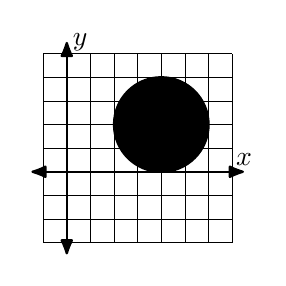
\begin{tikzpicture}[scale=0.3]

\fill [fill=\drawfill] (4,2) circle (2);

\draw [line width=0.1mm] (-1,-3) grid (7,5);
 
\draw[line width=0.3mm, <->, >={Latex[round]}] (-1.5, 0) -- (7.5, 0);

\draw[line width=0.3mm, <->, >={Latex[round]}] (0, -3.5) -- (0, 5.5);

\draw [black, line width=0.3mm] (4,2) circle (2);

\fill [fill=black] (4,2) circle (4pt);

\node[anchor=south, inner sep=2pt, rotate=0] (x-label) at (7.5,0) {$ x$};  

\node[anchor=west, inner sep=2pt, rotate=0] (y-label) at (0,5.5) {$ y$};  

\end{tikzpicture} 
%2
\item 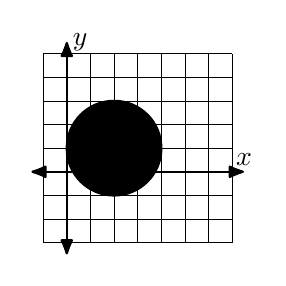
\begin{tikzpicture}[scale=0.3]

\fill [fill=\drawfill] (2,1) circle (2);

\draw [line width=0.1mm] (-1,-3) grid (7,5);
 
\draw[line width=0.3mm, <->, >={Latex[round]}] (-1.5, 0) -- (7.5, 0);

\draw[line width=0.3mm, <->, >={Latex[round]}] (0, -3.5) -- (0, 5.5);

\draw [black, line width=0.3mm] (2,1) circle (2);

\fill [fill=black] (2,1) circle (4pt);

\node[anchor=south, inner sep=2pt, rotate=0] (x-label) at (7.5,0) {$ x$};  

\node[anchor=west, inner sep=2pt, rotate=0] (y-label) at (0,5.5) {$ y$};  

\end{tikzpicture} 
%3
\item 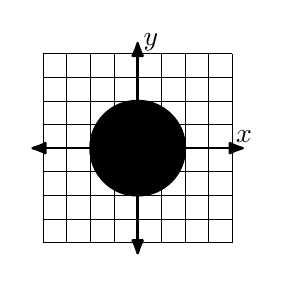
\begin{tikzpicture}[scale=0.3]

\fill [fill=\drawfill] (0,0) circle (2);

\draw [line width=0.1mm] (-4,-4) grid (4,4);
 
\draw[line width=0.3mm, <->, >={Latex[round]}] (-4.5, 0) -- (4.5, 0);

\draw[line width=0.3mm, <->, >={Latex[round]}] (0, -4.5) -- (0, 4.5);

\draw [black, line width=0.3mm] (0,0) circle (2);

\fill [fill=black] (0,0) circle (4pt);

\node[anchor=south, inner sep=2pt, rotate=0] (x-label) at (4.5,0) {$ x$};  

\node[anchor=west, inner sep=2pt, rotate=0] (y-label) at (0,4.5) {$ y$};  

\end{tikzpicture} 
%4
\item 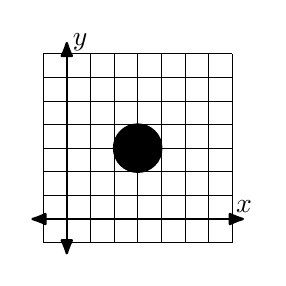
\begin{tikzpicture}[scale=0.3]

\fill [fill=\drawfill] (3,3) circle (1);

\draw [line width=0.1mm] (-1,-1) grid (7,7);
 
\draw[line width=0.3mm, <->, >={Latex[round]}] (-1.5, 0) -- (7.5, 0);

\draw[line width=0.3mm, <->, >={Latex[round]}] (0, -1.5) -- (0, 7.5);

\draw [black, line width=0.3mm] (3,3) circle (1);

\fill [fill=black] (3,3) circle (4pt);

\node[anchor=south, inner sep=2pt, rotate=0] (x-label) at (7.5,0) {$ x$};  

\node[anchor=west, inner sep=2pt, rotate=0] (y-label) at (0,7.5) {$ y$};  

\end{tikzpicture} 
%5 
\item 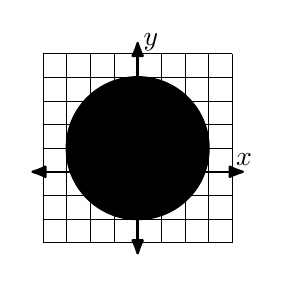
\begin{tikzpicture}[scale=0.3]

\fill [fill=\drawfill] (0,1) circle (3);

\draw [line width=0.1mm] (-4,-3) grid (4,5);
 
\draw[line width=0.3mm, <->, >={Latex[round]}] (-4.5, 0) -- (4.5, 0);

\draw[line width=0.3mm, <->, >={Latex[round]}] (0, -3.5) -- (0, 5.5);

\draw [black, line width=0.3mm] (0,1) circle (3);

\fill [fill=black] (0,1) circle (4pt);

\node[anchor=south, inner sep=2pt, rotate=0] (x-label) at (4.5,0) {$ x$};  

\node[anchor=west, inner sep=2pt, rotate=0] (y-label) at (0,5.5) {$ y$};  

\end{tikzpicture} 
%6
\item 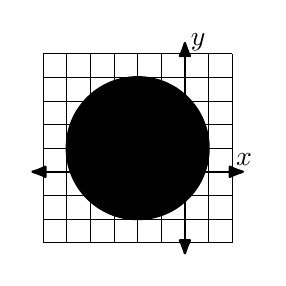
\begin{tikzpicture}[scale=0.3]

\fill [fill=\drawfill] (-2,1) circle (3);

\draw [line width=0.1mm] (-6,-3) grid (2,5);
 
\draw[line width=0.3mm, <->, >={Latex[round]}] (-6.5, 0) -- (2.5, 0);

\draw[line width=0.3mm, <->, >={Latex[round]}] (0, -3.5) -- (0, 5.5);

\draw [black, line width=0.3mm] (-2,1) circle (3);

\fill [fill=black] (-2,1) circle (4pt);

\node[anchor=south, inner sep=2pt, rotate=0] (x-label) at (2.5,0) {$ x$};  

\node[anchor=west, inner sep=2pt, rotate=0] (y-label) at (0,5.5) {$ y$};  

\end{tikzpicture} 
\end{multicols} 
\end{enumerate}  
%B
%\item \hspce 
%\begin{center}
\vspace*{1ex}
\scalebox{0.8}{
\noindent\begin{minipage}{\textwidth}
{

B. Find the center and radius of each circle with the given equation. 
\begin{enumerate}[label = \arabic*. ]
\begin{multicols}{2}

%1
\item \hspce $2x^2 + 2y^2 =32 $
%2
\item \hspce $x^2 + (y+5)^2 =100 $
%3
\item \hspce $(x-5)^2 + y^2 =169 $
%4
\item \hspce $(x+2)^2 + (y-4)^2 =36 $
%5 
%\item \hspce $(x-3)^2 + (y+2)^2 =16 $

\end{multicols} 
\end{enumerate}  
%C
%\item \hspce 
%end{enumerate}  
C. Write an equation of circle $C$ based on the given information. 
\begin{enumerate}[label = \arabic*. ]
%1
\item Center at (5, 4) and touching the x-axis 
%2
\item Center at (10, 4) and passing through (2, 2)
%3
\item Center at (3, 8) and passing through the origin 
%4
\item Center at (2, 5) and tangent to the y-axis
%5 
\item A circle with area 49 $\text{cm}^2 $ and center at (2, 5)
\end{enumerate}   

}
\end{minipage}}
%\end{center} 


%}} 

%\newpage

%{\fontsize{38}{40}\fontfamily{pnc}\selectfont {

%D
%\item 
%\begin{center}
\vspace*{1ex}
\scalebox{0.75}{
\noindent\begin{minipage}{\textwidth}
{
D. Write each equation of a circle in general form. 
\begin{enumerate}[label = \arabic*. ]
\begin{multicols}{2}

%1
\item \hspce  $(x-2)^2 + (y-4)^2 = 36$
%2
\item \hspce  $(x+4)^2 + (y-9)^2 = 144$
%3
\item  \hspce $(x-6)^2 + (y-1)^2 = 81$
%4
%\item \hspce  $(x-8)^2 + (y+7)^2 = 225$
%5 
\item \hspce  $x^2 + (y-5)^2 = 36$
\end{multicols} 
\end{enumerate}  

%E
%\item 
E. Transform each equation to standard form, then give the coordinates of the center and the radius. 
\begin{enumerate}[label = \arabic*. ]
\begin{multicols}{2}
%1
\item  $x^2 + y^2 -2x -8y -47 =0$
%2
\item  $x^2 + y^2 +4x -4y -28 =0$
%3
\item  $x^2 + y^2 +10x +4y -3 =0$
%4
\item  $x^2 + y^2 +8y -84 =0$
%5 
%\item \hspce $x^2 + y^2 +8x -6y -39 =0$
\end{multicols} 
\end{enumerate}  
}
\end{minipage}}
%\end{center}  
\vspace*{1ex}
}}
\newpage

{\fontsize{36}{40}\fontfamily{pnc}\selectfont {
\def\curdir{/storage/emulated/0/Documents/documents/latex/1920/Grade-10/3rd/equation-and-graph-of-a-circle/fb}

%\textbf{Practice Exercises}
\textbf{Problem Set}

\vspce

%\begin{enumerate}[label = \Alph*. ]
%A
%\item \hspce
A. Give the radius and coordinates of the center of the circle. Then write the equation in standard form. 
\begin{enumerate}[label = \arabic*. ]

\begin{multicols}{3}
%1 
\item 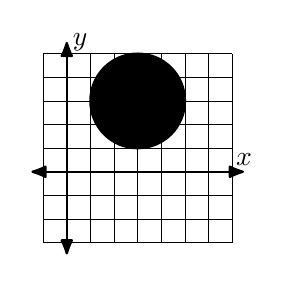
\begin{tikzpicture}[scale=0.3]

\filldraw [fill=\drawfill, line width=0.3mm] (3,3) circle (2);

\draw [line width=0.1mm] (-1,-3) grid (7,5);
 
\draw[line width=0.3mm, <->, >={Latex[round]}] (-1.5, 0) -- (7.5, 0);

\draw[line width=0.3mm, <->, >={Latex[round]}] (0, -3.5) -- (0, 5.5);

%\fill [opacity=.5,fill=\drawfill] (4,2) circle (2);

\fill [fill=black] (3,3) circle (4pt);

\node[anchor=south, inner sep=2pt, rotate=0] (x-label) at (7.5,0) {$ x$};  

\node[anchor=west, inner sep=2pt, rotate=0] (y-label) at (0,5.5) {$ y$};  

\end{tikzpicture} 
%2
\item 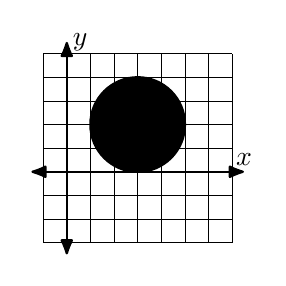
\begin{tikzpicture}[scale=0.3]

\filldraw [fill=\drawfill, line width=0.3mm] (3,2) circle (2);

\fill [fill=black] (3,2) circle (4pt);

\draw [line width=0.1mm] (-1,-3) grid (7,5);
 
\draw[line width=0.3mm, <->, >={Latex[round]}] (-1.5, 0) -- (7.5, 0);

\draw[line width=0.3mm, <->, >={Latex[round]}] (0, -3.5) -- (0, 5.5);

\node[anchor=south, inner sep=2pt, rotate=0] (x-label) at (7.5,0) {$ x$};  

\node[anchor=west, inner sep=2pt, rotate=0] (y-label) at (0,5.5) {$ y$};  

\end{tikzpicture} 
%3
\item 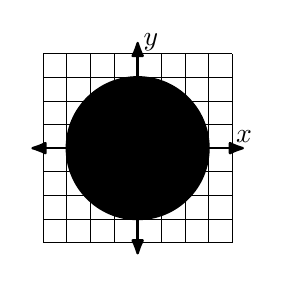
\begin{tikzpicture}[scale=0.3]

\filldraw [fill=\drawfill, line width=0.3mm] (0,0) circle (3);

\fill [fill=black] (0,0) circle (4pt);

\draw [line width=0.1mm] (-4,-4) grid (4,4);
 
\draw[line width=0.3mm, <->, >={Latex[round]}] (-4.5, 0) -- (4.5, 0);

\draw[line width=0.3mm, <->, >={Latex[round]}] (0, -4.5) -- (0, 4.5);

\node[anchor=south, inner sep=2pt, rotate=0] (x-label) at (4.5,0) {$ x$};  

\node[anchor=west, inner sep=2pt, rotate=0] (y-label) at (0,4.5) {$ y$};  

\end{tikzpicture} 
%4
\item 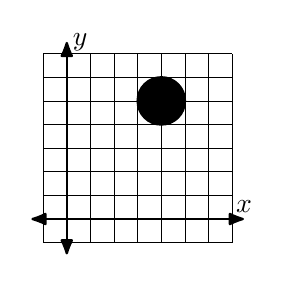
\begin{tikzpicture}[scale=0.3]

\filldraw [fill=\drawfill, line width=0.3mm] (4,5) circle (1);

\fill [fill=black] (4,5) circle (4pt);

\draw [line width=0.1mm] (-1,-1) grid (7,7);
 
\draw[line width=0.3mm, <->, >={Latex[round]}] (-1.5, 0) -- (7.5, 0);

\draw[line width=0.3mm, <->, >={Latex[round]}] (0, -1.5) -- (0, 7.5);

\node[anchor=south, inner sep=2pt, rotate=0] (x-label) at (7.5,0) {$ x$};  

\node[anchor=west, inner sep=2pt, rotate=0] (y-label) at (0,7.5) {$ y$};  

\end{tikzpicture} 
%5 
\item 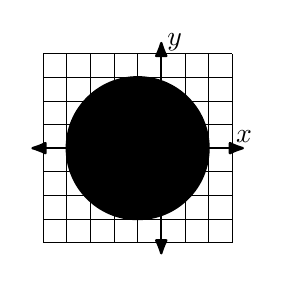
\begin{tikzpicture}[scale=0.3]

\filldraw [fill=\drawfill, line width=0.3mm] (-1,0) circle (3);

\fill [fill=black] (-1,0) circle (4pt);

\draw [line width=0.1mm] (-5,-4) grid (3,4);
 
\draw[line width=0.3mm, <->, >={Latex[round]}] (-5.5, 0) -- (3.5, 0);

\draw[line width=0.3mm, <->, >={Latex[round]}] (0, -4.5) -- (0, 4.5);

\node[anchor=south, inner sep=2pt, rotate=0] (x-label) at (3.5,0) {$ x$};  

\node[anchor=west, inner sep=2pt, rotate=0] (y-label) at (0,4.5) {$ y$};  

\end{tikzpicture} 
%6
\item 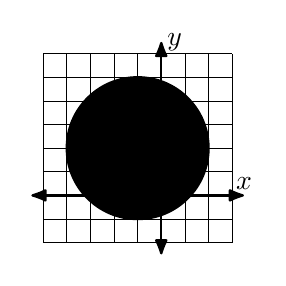
\begin{tikzpicture}[scale=0.3]

\filldraw [fill=\drawfill, line width=0.3mm] (-1,2) circle (3);

\fill [fill=black] (-1,2) circle (4pt);

\draw [line width=0.1mm] (-5,-2) grid (3,6);
 
\draw[line width=0.3mm, <->, >={Latex[round]}] (-5.5, 0) -- (3.5, 0);

\draw[line width=0.3mm, <->, >={Latex[round]}] (0, -2.5) -- (0, 6.5);

\node[anchor=south, inner sep=2pt, rotate=0] (x-label) at (3.5,0) {$ x$};  

\node[anchor=west, inner sep=2pt, rotate=0] (y-label) at (0,6.5) {$ y$};  


\end{tikzpicture} 
\end{multicols} 
\end{enumerate}  
%B
%\item \hspce 
%\begin{center}
%\vspace*{-2ex}
\scalebox{0.75}{
\noindent\begin{minipage}{\textwidth}
{
B. Find the center and radius of each circle with the given equation. 
\begin{enumerate}[label = \arabic*. ]
\begin{multicols}{2}
%1
\item \hspce $3x^2 + 3y^2 =12 $
%2
\item \hspce $x^2 + (y+4)^2 =81 $
%3
\item \hspce $(x-3)^2 + y^2 =144 $
%4
\item \hspce $(x+4)^2 + (y-3)^2 =64 $
%5 
%\item \hspce $(x-5)^2 + (y+1)^2 =49 $
\end{multicols} 
\end{enumerate}  
%C
%\item \hspce 
C. Write an equation of circle $C$ based on the given information. 
\begin{enumerate}[label = \arabic*. ]
%1
\item Center at (3, 2) and touching the x-axis 
%2
\item Center at (7, 5) and passing through (3, 4)
%3
\item Center at (4, 7) and passing through the origin 
%4
\item Center at (3, 7) and tangent to the y-axis
%5 
\item A circle with area 64 $\text{cm}^2 $ and center at (3, 6)
\end{enumerate}   

%D
%\item 
D. Write each equation of a circle in general form. 
\begin{enumerate}[label = \arabic*. ]
\begin{multicols}{2}
%1
\item \hspce  $(x-7)^2 + y^2 = 64$
%2
\item \hspce  $x^2 + (y+2)^2 = 49$
%3
\item  \hspce $(x+2)^2 + y^2 = 100$
%4
\item \hspce  $(x-5)^2 + (y-5)^2 = 27$
%5 
%\item \hspce  $(x+4)^2 + (y+4)^2 = 32$
\end{multicols} 
\end{enumerate}  

%E
%\item 
E. Transform each equation to standard form, then give the coordinates of the center and the radius. 
\begin{enumerate}[label = \arabic*. ]
\begin{multicols}{2}
%1
\item  $x^2 + y^2 -8x +2y -32 =0$
%2
\item   $x^2 + y^2 -6x -10y +18 =0$
%3
\item  $x^2 + y^2 - 6 x - 2 y - 15=0$
%4
\item  $x^2 + y^2 - 4 x + 6 y + 4 =0$
%5 
%\item \hspce $x^2 + y^2- 2 x  + 8 y - 47 =0$
\end{multicols} 
\end{enumerate}  

%\end{enumerate}  
}
\end{minipage}}
%\end{center}  


}}
\newpage

{\fontsize{36}{40}\fontfamily{pnc}\selectfont {
\input{ps-equation-and-graph-of-a-circle-sol}

}}

\end{document}